\section{Discussion}
\graphicspath{{Figures/}{../Figures/}}
\label{Discussion}
 As mentioned previously, there are many cited models touted by the press and scientific community.  The most popular one seems to be the Institute for Health Metrics and Evaluation (IHME) model \cite{imhe}.  This model has been considerably under-predicting projected death counts over the iterations of the model.  There are several assumptions at play that make this model questionable.  First, they assume a symmetric Gaussian-like curve for daily deaths and therefore a sigmoid-like curve for cumulative deaths.  There are epidemiological models that support this, but it remains to be seen if this will apply to different countries following different containment measures. Going back to smallpox outbreaks of the 1840's, William Farr showed that epidemics rise and fall in roughly a bell-shaped curve \cite{farr}.  Additionally, Farr stated topically that "The death rate is a fact; anything beyond this is an inference".  
 
 Assuming a Gaussian-like curve, we should expect to see shapes shown in Figure \ref{m3} when analyzing infections and deaths.

 \begin{figure}[H]
\centerline{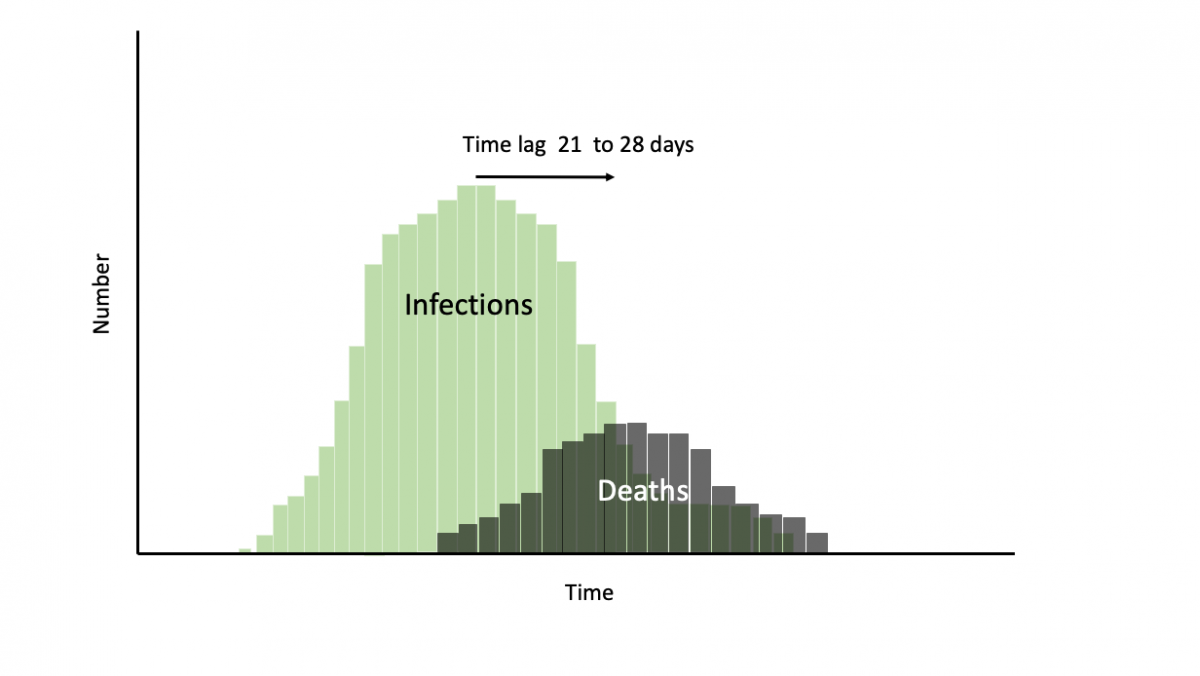
\includegraphics[scale=0.18]{Figures/ss.png}}
\caption{Gaussian-like Approach of Modeling COVID-19}
\label{m3}
\end{figure}


However, when compared to the actual shapes of Italy, a smooth curve is not seen.  It seems to more plateau rather than sharply decline as fast as it rose as shown in Figure \ref{m4}.

 
 \begin{figure}[H]
\centerline{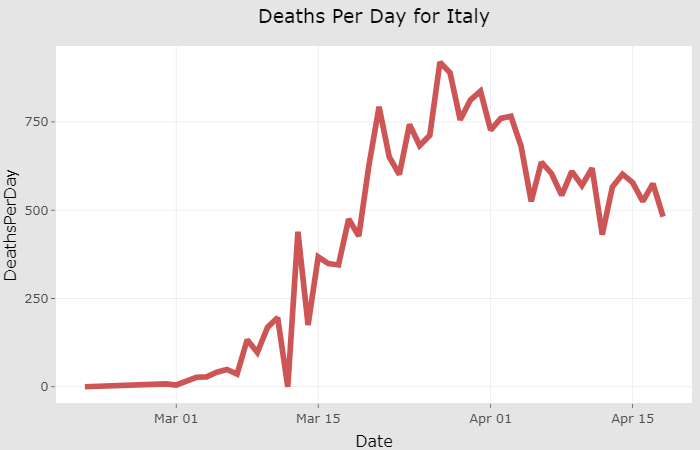
\includegraphics[scale=0.30]{Figures/newplot.png}}
\caption{Italy COVID Deaths Per Day}
\label{m4}
\end{figure}


For Italy and Spain, IHME estimates are passing outside their confidence bounds over the past iterations.  Predictive models that fail to predict two days out within a 95 percent confidence interval are not adequate to model such an important problem. Another caveat of this model is that it is fitted using data from Wuhan which sharply and questionably goes down to 0.  It also fits on data from other countries that are following social distancing and quarantine much more seriously than the United States. Perhaps America's greatest strength is also our greatest weakness when it comes to pandemics, and our quest for freedom and civil liberties are antithetical to containing this disease.
 
 Other models have similar drawbacks.  Notably, the CovidActNow model over-forecasts in the other direction.  It assumes very high R\typesubscript{0} with social distancing, inflating future fatalities and the spread of the disease.  With reported R\typesubscript{0} of under 1 in New York, it is hard to believe their initial assumed 2.1 R\typesubscript{0} is accurate.  Additionally, the CovidActNow model is focused on modeling the disease with assumptions rather than curve fitting.  The Los Alamos National Lab Forecasting team's model has performed the most accurately of all discussed models.  The strengths of the Los Alamos model is that they do not make any assumptions about R\typesubscript{0} except that it will eventually trend downwards. Next they randomly sample all possibilities of the growth rate over time to achieve their forecast.  
 
 \begin{figure}[H]
\centerline{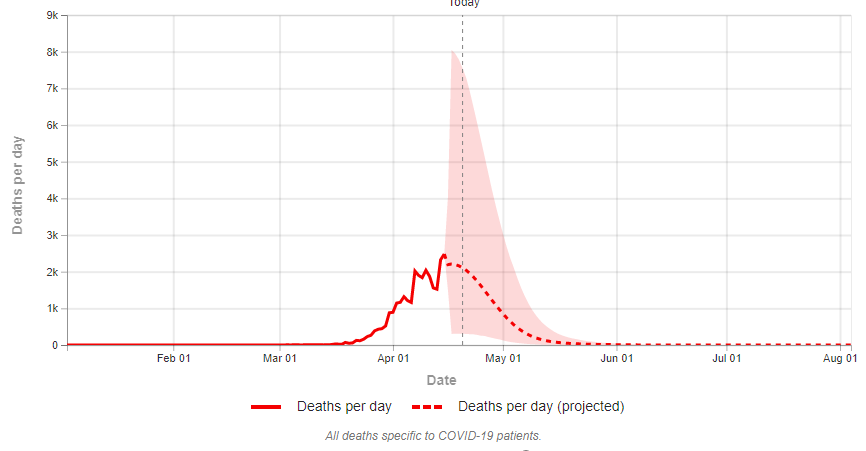
\includegraphics[scale=0.35]{Figures/2.PNG}}
\caption{IMHE Daily Death Model}
\label{m4}
\end{figure}